\documentclass[12pt]{article}
\usepackage{pdfpages}
\usepackage{tabularx}
\usepackage[utf8]{inputenc}
\usepackage{geometry}
\usepackage{a4wide}
\usepackage{graphicx}
\usepackage[style=authoryear,backend=biber]{biblatex}
\usepackage{ragged2e}  % for '\RaggedRight' macro (allows hyphenation)

\newcolumntype{Y}{>{\RaggedRight\arraybackslash}X}

\geometry{\
 a4paper,
 total={170mm,257mm},
 left=20mm,right=20mm,
 top=20mm, bottom=25mm
 }

\graphicspath{{images/}}

\addbibresource{biblio.bib}

\title{Scoping And Planning Document}
\date{November 2017}

\usepackage{setspace}
\usepackage{listings}
\usepackage{geometry}
\usepackage[toc,page]{appendix}
\usepackage{booktabs}
\usepackage{multirow}
\usepackage{lipsum}
\usepackage[export]{adjustbox}
\usepackage[T1]{fontenc}
\usepackage{textcomp}
\usepackage{epsfig,graphics}
\usepackage{graphicx}
\usepackage{amssymb}
\usepackage{titlesec}
\usepackage[justification=centering]{caption}
\usepackage{chngcntr}
\usepackage[section]{placeins}
\usepackage{amsmath}
\usepackage[style=numeric,backend=biber,sorting=none]{biblatex}
\usepackage{enumitem}
\usepackage{pgfgantt}
\usepackage{lscape}
\usepackage[parfill]{parskip}
\usepackage[utf8]{inputenc}
\usepackage[T1]{fontenc}
\usepackage{subfig}

\graphicspath{{images/}}
\counterwithout{figure}{chapter}
\addbibresource{refs.bib}

%%%%%%%%%%%%%%%%%%%%%%%%%%%%%%%%%%%%%%%%%%%%%%%%%%%%%%%%%%%%%%%%%%%%%%%%%%%%%%
% Details of project
%%%%%%%%%%%%%%%%%%%%%%%%%%%%%%%%%%%%%%%%%%%%%%%%%%%%%%%%%%%%%%%%%%%%%%%%%%%%%%
\newcommand{\projectTitle}{Reinforcement Learning For Games: An Intelligent
Agent for StarCraft II}
\newcommand{\fullname}{Amir Faris, Daniel Spooner, Ryan Cross}
\newcommand{\degreeTitle}{MEng Computer Science}
\newcommand{\session}{2017--2018}
\newcommand{\by}{$\times$}

%%%%%%%%%%%%%%%%%%%%%%%%%%%%%%%%%%%%%%%%%%%%%%%%%%%%%%%%%%%%%%%%%%%%%%%%%%%%%%
% Change the geometry of the page to have a 25 mm binding edge
%%%%%%%%%%%%%%%%%%%%%%%%%%%%%%%%%%%%%%%%%%%%%%%%%%%%%%%%%%%%%%%%%%%%%%%%%%%%%%
\geometry{%
    a4paper,
    total={210mm,297mm},
    left=25mm,
    right=25mm,
    top=25mm,
    bottom=20mm,
}

%%%%%%%%%%%%%%%%%%%%%%%%%%%%%%%%%%%%%%%%%%%%%%%%%%%%%%%%%%%%%%%%%%%%%%%%%%%%%%
% Commands to set the line spacing
%%%%%%%%%%%%%%%%%%%%%%%%%%%%%%%%%%%%%%%%%%%%%%%%%%%%%%%%%%%%%%%%%%%%%%%%%%%%%%
%\singlespacing\
\onehalfspacing%
%\doublespacing\

%%%%%%%%%%%%%%%%%%%%%%%%%%%%%%%%%%%%%%%%%%%%%%%%%%%%%%%%%%%%%%%%%%%%%%%%%%%%%%
% Spacing for the chapter header
%%%%%%%%%%%%%%%%%%%%%%%%%%%%%%%%%%%%%%%%%%%%%%%%%%%%%%%%%%%%%%%%%%%%%%%%%%%%%%
\titleformat{\chapter}[display]
    {\normalfont\Huge\bfseries}{\vspace*{-1\baselineskip}\chaptertitlename\ \thechapter}{15pt}{\huge}
\titlespacing*{\chapter}{0pt}{0pt}{15pt}

\renewcommand\bibname{References}

%%%%%%%%%%%%%%%%%%%%%%%%%%%%%%%%%%%%%%%%%%%%%%%%%%%%%%%%%%%%%%%%%%%%%%%%%%%%%%
% Some shortcuts that maybe useful
%%%%%%%%%%%%%%%%%%%%%%%%%%%%%%%%%%%%%%%%%%%%%%%%%%%%%%%%%%%%%%%%%%%%%%%%%%%%%%
\DeclareTextCommandDefault{\textcopyright}{\textcircled{c}}
\newcommand*\rot{\rotatebox{90}}

%%%%%%%%%%%%%%%%%%%%%%%%%%%%%%%%%%%%%%%%%%%%%%%%%%%%%%%%%%%%%%%%%%%%%%%%%%%%%%
% Bibliography style: choose one and make sure you have the relevant .bst file
%%%%%%%%%%%%%%%%%%%%%%%%%%%%%%%%%%%%%%%%%%%%%%%%%%%%%%%%%%%%%%%%%%%%%%%%%%%%%%
%\bibliographystyle{abbrv}

%%%%%%%%%%%%%%%%%%%%%%%%%%%%%%%%%%%%%%%%%%%%%%%%%%%%%%%%%%%%%%%%%%%%%%%%%%%%%%
% Layout for the front cover !!!!! YOU SHOULD NOT HAVE TO CHANGE THIS!!!!!
%%%%%%%%%%%%%%%%%%%%%%%%%%%%%%%%%%%%%%%%%%%%%%%%%%%%%%%%%%%%%%%%%%%%%%%%%%%%%%

\newcommand{\frontcover}{
    % The title page:
    \begin{titlepage}
        \newgeometry{left=25mm,right=25mm,top=45mm,bottom=0.1cm}

        \begin{minipage}[t]{7cm}
            \noindent\textbf{\Large{School of Computing}}\\
            {\fontfamily{ptm}\selectfont 
                \uppercase{faculty of engineering}
            }
        \end{minipage}
        \hfill
        \begin{minipage}[t]{7cm}
            \vspace*{-25pt}
            
\includegraphics[scale=0.2,right]{logo_black.png}
            \vspace*{-1pt}
        \end{minipage}

        \noindent\makebox[\linewidth]{\rule{\paperwidth}{0.4pt}}

        \centering
        \vspace*{37mm}
        \textbf{\Large\projectTitle}\\
        \vspace*{10mm}
        \textbf{\large\fullname}\\
        \vspace*{10mm}
        \textbf{Submitted in accordance with the requirements for the masters of}\\
        \textbf{\degreeTitle}\\
        \vspace*{10mm}
        \session\\
        \restoregeometry%
    \end{titlepage}
}

%%%%%%%%%%%%%%%%%%%%%%%%%%%%%%%%%%%%%%%%%%%%%%%%%%%%%%%%%%%%%%%%%%%%%%%%%%%%%%
% Define a new environment for the dissertation summary
%%%%%%%%%%%%%%%%%%%%%%%%%%%%%%%%%%%%%%%%%%%%%%%%%%%%%%%%%%%%%%%%%%%%%%%%%%%%%%
\newenvironment{dissertationsummary}
{\cleardoublepage\ \null\
    \begin{center}%
        \textbf{Summary}
\end{center}}%
{\vfill \null}


\begin{document}
\pagenumbering{gobble}
\begin{minipage}[t]{90mm}
\flushleft
\Huge{\textbf{School of Computing}}
\end{minipage}
\hfill\hfill
\begin{minipage}[t]{70mm}
\flushright

\includegraphics{Leeds_BLACK}
\end{minipage}


\begin{center}
\LARGE{\modulecode}\\
\normalsize{\textbf{Scoping and Planning Document}}
\end{center}

\begin{tabularx}{\textwidth}{|Y|}
\hline
\vspace*{0.005\textheight} \textbf{Student Name}: \fullname \vspace*{0.01\textheight}\\ \hline
\vspace*{0.005\textheight} \textbf{Programme of Study}: \PoS  \vspace*{0.01\textheight}\\ \hline
\vspace*{0.005\textheight} \textbf{Provisional Title of Project}: \ProjectTitle \vspace*{0.01\textheight}\\ \hline
\vspace*{0.005\textheight} \textbf{Name of External Company} \tiny{(if applicable})\normalsize: \CN \vspace*{0.01\textheight}\\ \hline
\vspace*{0.005\textheight} \textbf{Supervisor Name}: \Supervisor \vspace*{0.01\textheight}\\ \hline
\vspace*{0.005\textheight} \textbf{Type of Project}: \ToP \vspace*{0.01\textheight}\\ \hline
\vspace*{0.005\textheight}\textbf{Note to student}: ensure you have discussed the content with the supervisor well in advanced of the dealine for submission. Submit a \textbf{hard copy} to the SSO. An \textbf{electronic version} of this report in pdf must also be submitted via the appropriate module folder in the VLE; with filename $<$surname$><$year$>$-SP.pdf. \vspace*{0.01\textheight}\vspace*{0.01\textheight}\\ \hline
\vspace*{0.005\textheight} \textbf{Signature of Student}:\vspace*{0.05\textheight}   \\ \hline 
\vspace*{0.005\textheight} \textbf{Date}:\vspace*{0.01\textheight}\\ \hline

\vspace*{0.005\textheight}\textbf{Assessor} \tiny{(leave blank)}:\\ \vspace*{0.1\textheight} \normalsize NOTE to assessor: feedback form is available to download from the VLE resources `Quick Links'.On completion, please attach the feedback form to this document and return to the SSO. \\ \hline
\end{tabularx}
\newpage
\tableofcontents
\newpage
\pagenumbering{arabic}

\maketitle

\section{Background Research for the Project}

The project deals with the use of machine learning algorithms in a game space.
The game in use is StarCraft 2 and will be implemented using the StarCraft 2
Learning Environment developed by Blizzard and Google.
The project deals with feasible implementations of machine learning within
StarCraft 2 with an emphasis on accuracy and speed over complexity and
flexibility.

\subsection{Context}
Recently AI research has been conquering extremely complex games such as
Chess and Go (\cite{deepmind}). These games involve in-depth strategy decision
making but have some aspects in common: The domain is set and unchanging
(the game board), the game is turn-based and players have full knowledge of
the game (they can see all the board and all pieces).
The next step in AI research of this type is to look at problems that expand
beyond these limitations; computer games offer a new challenge as they
do not have to rely on turn-based gameplay (\textcite{vinyals2017starcraft}).
All agents (human or machine) can act simultaneously on the world in real time;
this dramatically increases
the speed at which an AI must think and react to the problem presented.
In addition, many computer games rely on presenting an incomplete version
of the world, deliberately hiding information from the players so reasoning
must be done without full knowledge of the possible consequences.
StarCraft 2 created by Blizzard Entertainment is a Real-Time Strategy (RTS)
game (\cite{starcraft2}). It is considered an ideal candidate for this type of
AI work because it combines deep strategy, real-time combat and partial
world obscuration. Another exciting aspect of StarCraft 2, in particular,
is the possible asymmetry in gameplay; In chess, both players have
identical pieces but in StarCraft players can pick from 3 different
races each of which has substantially different gameplay mechanics and units.
Because of all these additional challenges mastering the whole game is
beyond the remit of this project, so a smaller subset of the problem
will be created using in-game tools to work with.

\subsection{Problem Statement}

To create a simple map with a single unit to control.
This unit will be presented the task of moving across the map to a
pre-arranged destination dealing with any hazards in place.
The difficulty of the problem to start with will be a simple navigation
problem, that we then expand as the AI progresses in learning. The
method of learning will also influence the agent and will develop different
behaviours based on the learning pattern. The agent would also need to be
able to apply what it was taught in different environments and adapt
accordingly. Furthermore, training time can also be an issue since the
amount of time needed for the agent to learn a particular behaviour will vary.
The complexity of the game raises major issues in implementation, the agent
may only be able to achieve a small subset of the task, such as reaching the
tower but not destroying it. The controls for agent movement would also give rise
to more issues with how well can the character be controlled and what are the
parameters the agent needs to achieve simple movement.
Different characters mean that different agents would be required to
achieve different playing patterns that best fit the given character.

\subsection{Possible Solution}

A solution to this problem will include a number of different
components. For starters, it will require an interface with
the DeepMind StarCraft 2 Learning Environment
(\cite{pysc2}),
such that our agent may interface with the game.
Next, we will need a number of maps that the agent may train
on and be tested in.

Most importantly, will be the model we use for the agent itself.
The agent should be able to act intelligently on the maps it was
tested with, and hopefully be able to generalise somewhat
to secondary challenges.

\subsection{Quality of Solution}
The following define the quality of the solution:
\begin{itemize}
    \item How fast can an agent be taught to achieve the required task?
    \item How effective is the agent’s current ability to solve
          the given the task?
    \item Did the agent find the optimal solution or something
          within an acceptable threshold?
\end{itemize}

The agent should able to achieve the given objective within a reasonable
time frame that is defined by the given task. To achieve this the agent
will be put through multiple learning scenarios and expected to improve
with each iteration. The ideal solution would depend on the learning
rate of the agent and the agent’s ability to perform in different
environments.

Finding an optimal path with the given environment will differ
based on the structure and complexity of the level. The agent should
find a route that is reasonable and near the optimal path
to the target goal of the level.

\section{Scope of the Project}

\subsection{Aim}
To apply machine learning techniques within the StarCraft 2 engine.
Using a custom designed map as the problem space,
the challenge should include navigation of the map,
tackling hazards and reaching an objective point.

\subsection{Objectives}
Our objectives are as follows:
\begin{itemize}
    \item An underlying interface with the SC2 API capable of providing
          information to the agent and receiving action instructions
          from it to control the game.

          To work on the machine learning, a stable interface between the
          game software and our own is necessary. This interface will present
          a model of the game world to the agent that it can interact with,
          reading information and using predefined actions to
          operate within the represented world.
    \item SC2 maps designed for the agent to run on.

          StarCraft 2 is an extremely complicated game,
          so a lot of machine learning research instead choose to run
          on a restricted version of the game. Because of this,
          we will need several custom maps that we can both train our
          agent in, as well as test its performance. This will be
          achieved with StarCraft 2’s extensive tool kit that can
          be used to create custom maps within the game.
          These tools will be utilised to create the environments for
          our agent to train and work within. Because the maps are
          so customisable we will be able to update them as needed to
          test various aspects of the AI.

    \item A prototype used for training the agent, possibly across a few
          different training techniques.

          The main objective of this project is to have an intelligent
          agent that can perform tasks. Because of this, we will need to build
          up a prototype for the agent, in both how it learns and how that
          learning is passed through to and from the SC2 API, from the
          first objective.

    \item Documentation describing the programming including user instructions.

          Clear information on the design and operation of the software including
          instructions for installation and running of the program.
          This will also include in-depth information on the programming its
          self to aid in understand of its functionality and provide help with
          further adaptation by 3rd parties.

    \item Analysis of the agent. Effectiveness, efficiency and completeness.

          Once we have an agent that exhibits intelligent behaviour in our maps,
          we will need to formally test its capabilities in several areas, so
          that we may compare the agent against other prototypes, those
          which were trained under different parameters, or under a different
          learning type potentially. Of note, we are interested in the speed
          of learning, that is how many iterations does it take to reach an
          intelligent solution, the efficiency of the solution, such that the
          agent isn’t performing un-needed tasks, and finally the
          complexity of environment the agent can deal with.

          Furthermore, depending on the task we choose, we may be able to
          compare against the basic agents that are included in the
          \cite{pysc2} environment, such that we can compare their progress
          and their intelligence, since they use more traditional techniques,
          such as greedy algorithms.

    \item A written report, to go alongside the prototype.

          This report will include the analysis as well as the research that
          went into the project and the implementation we settled on.
          This will allow the reader to understand why certain design
          decision were used, as well as the path we took to get there.
          This will further be augmented with personal log books,
          detailing what work went into the project, on a day-by-day basis.

    \item Possible Extension: To use transfer learning to move the agent’s
          learnt behaviour to an unfamiliar environment.

          This would allow us to apply newer research techniques,
          to see how they work as well as how they compare against
          more traditional models.
\end{itemize}

\subsection{Deliverables}
Our deliverables are as follows:
\begin{itemize}
    \item A prototype of the intelligent agent.
          This will include both the model and the trained values,
          to reproduce the results we achieve. This covers objectives 1, 3 and 7.
    \item The custom StarCraft 2 maps used for training and testing the agents,
          which fulfils objective 2, and allows our work to be reproduced more easily.
    \item Documentation for the system, in the form of a readme or Wiki,
          in a Git repo alongside the agent prototype, to cover objective 4.
    \item The individual report will contain both the analysis of the agent or
          agents we create, as well as the research that went into the prototype.
          This covers objective 6, and is also the deliverable of the most interest,
          as it should outline the whole project and inform the reader why design
          decisions were made, and the research that led to them being taken.
    \item Finally, Individual Reports and logbooks which will outline what each
          team member did on an individual day, and a retrospective on the project.
\end{itemize}

\section{Project Schedule}

There is 15 weeks total work time, 3 before Christmas, 12 after.
The first 3-week run will be done up to the 4th of December and will focus
on setting up the SC2 API within python with a minimal interaction, to
have an agent traverse the space of a simple map.

The next part of the project is scheduled to start from the 22nd of
January and is focused on applying learning methods and techniques
to the basic implementation we have.

Before Christmas we are aiming to have the API interface setup with
a basic agent interaction. If this proves easy, we can also do the
initial map design and start the research into possible approaches early
but otherwise these tasks will be done over the Winter break.

Once we are back, the next issue to tackle would be creating a minimal
environment that would be simple for the agent to learn on but would also
require the agent to use specific methods to complete the level. The level
designs will be done at the end of each successful iteration. Due to the
ambiguous nature of the agent’s ability to pick up habits of movement,
levels would have to be redesigned for an optimal solution to be accessible
to the agent. Each iteration will focus on breaking the project into more
complex tasks and will require further improvement to the learning aspect of
the agent. Once a level has been designed, the work would shift into
implementing a learning agent into said level. The agent is then trained
on the current level and will be tested for performance given that it has
learned the optimal solution. The development time is split into a learning
phase and a testing phase. The learning phase will be done in a single month bulk.

\subsection{Methodology}

Due to the nature of the task it is not possible to set a specific, well
defined end goal. Because of this an iterative development style will be adopted.
Initially work will focus upon base infrastructure such as interfacing with
the StarCraft API and creating a basic agent using statistical techniques.
As the project progresses time will be split into stages of in determinant length,
each stage will add additional features then be tested and reviewed.
The stage review will inform the goals for the next iteration.

\subsection{Tasks, Milestones and Timeline}

\begin{figure}[h]
    \hspace*{-1cm}\
    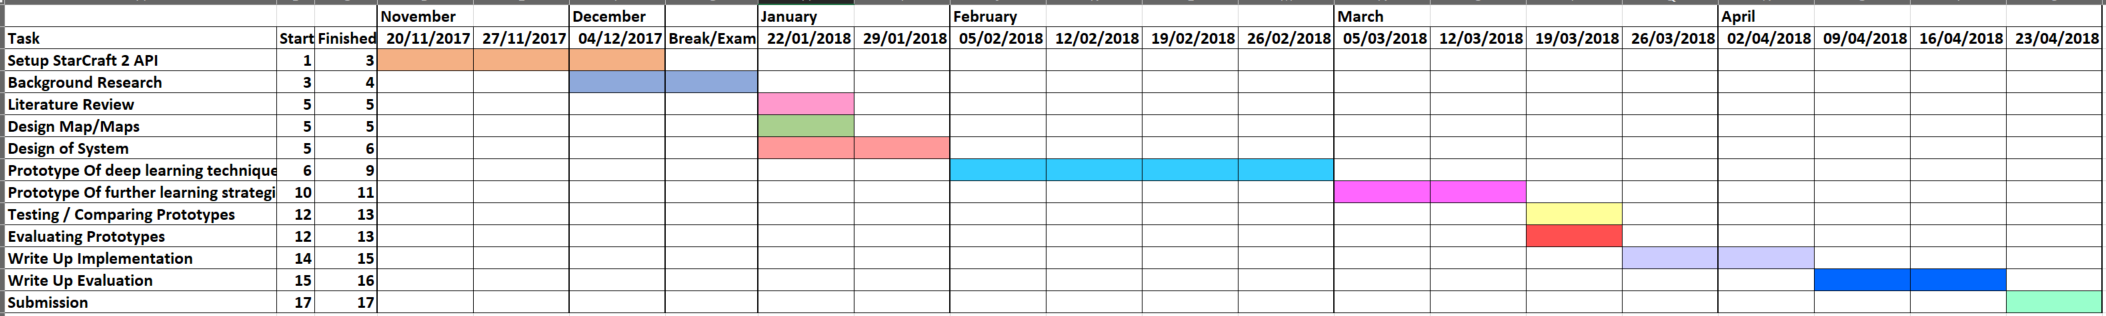
\includegraphics[width=1.1\textwidth]{gantt.png}
    \caption{Gantt Chart showing Timeline}
\end{figure}

\subsection{Risk Assessment}

\appendix
\section{Ethical Issues}
The project aims to create a specialised AI designed to solve an artificial
problem with no direct real-world applications.
No specific ethical concerns are foreseen or expected within the scope of the
planned design.

\printbibliography{}

\end{document}
